El experimento Solenoide Compacto de Muones o \CMS(\textbf{C}ompact \textbf{M}uon \textbf{S}olenoid) tiene la capacidad de cubrir un amplio rango de procesos físicos, este experimento consiste de varios subsistemas los cuales están diseñados para la identificación de prácticamente todas las partículas del modelo estándar. Para su diseño se tomó en cuenta cómo cada partícula interacciona con la materia, por ejemplo las partículas cargadas son identificadas por medio de detectores a base de silicio y de gas noble, permitiendo determinar con precisión el tiempo y localización de las partículas. La variedad de interacciones por tipo de partícula se puede ver en la Fig. \ref{cms}.

\begin{figure}[!ht]
\centering
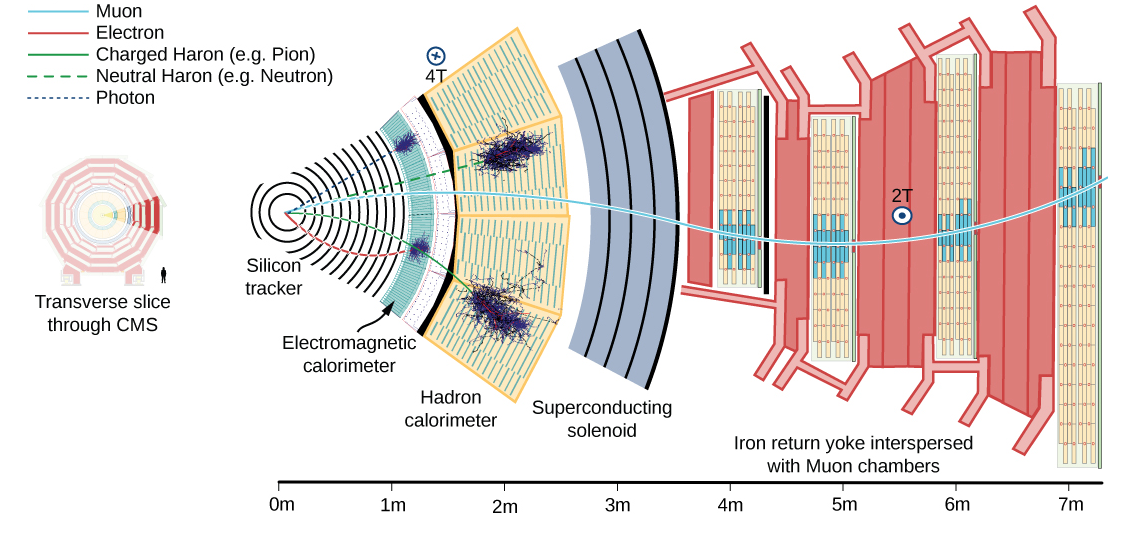
\includegraphics[width=1\textwidth]{Cap2/imagenes/CMS_interaction.png}
\caption[Detector de solenoide de muón compacto. El detector consta de varias capas, cada una responsable de medir diferentes tipos de partículas.]{Detector de solenoide de muón compacto. El detector consta de varias capas, cada una responsable de medir diferentes tipos de partículas.\footnotemark}
\label{cms}
\end{figure}

\footnotetext{Página de origen: \href{http://ippog.web.cern.ch/resources/2011/cms-slice-july-2010-version}{http://ippog.\-web.\-cern.\-ch/\-resources/\-2011/\-cms-\-slice-\-july-\-2010-\-version}}

El \CMS ~ es un detector de propósito general, capaz de estudiar múltiples aspectos de las colisiones de protones hasta 14 TeV, este contiene sistemas para medir la energía y la cantidad de movimiento de fotones, electrones, muones y otras partículas producto de las colisiones \citep{cms_1}. La capa detectoras (ver Fig. \ref{cms}) se pueden dividir en: 
\begin{itemize}
\item  \textbf{El detector de trazas de Silicio (The Silicon tracker):} para calcular el momento de una partícula es rastrear su camino a través de un campo magnético; ~ cuanto más curvaba el camino, menos impulso tenía la partícula. El detector de trazas \CMS ~ registra los caminos tomados por las partículas cargadas al encontrar sus posiciones en varios puntos clave. De esta forma se reconstruyen los caminos de muones de alta energía, electrones y hadrones (partículas formadas por quarks), así como ver las huellas que provienen de la descomposición de partículas de vida muy corta.

El detector de trazas \CMS ~ está hecho completamente de silicio: los píxeles, en el núcleo mismo del detector y que se ocupan de la mayor intensidad de partículas, y los detectores de microstrip de silicio que lo rodean. A medida que las partículas viajan a través del detector, los píxeles y las microstrips producen pequeñas señales eléctricas que se amplifican y detectan. %El rastreador emplea sensores que cubren un área del tamaño de una cancha de tenis, con 75 millones de canales de lectura electrónica separados: en el detector de píxeles hay unas 6,000 conexiones por centímetro cuadrado.

%\textbf{Actualización de Alta Luminosidad: }

%La actualización esperada de \textbf{HL-}\LHC~ aumentará el número de interacciones hasta el punto en que la ocupación excesiva reduciría significativamente la efectividad de la búsqueda de pistas. Se planea una actualización para aumentar el rendimiento y la tolerancia a la radiación del rastreador.

\item \textbf{Calorímetro electromagnético} o \textbf{ECAL} (\textbf{E}lectromagnetic \textbf{CAL}orimeter): componente diseñado para medir con alta precisión las energías de electrones y fotones, está construido a partir de cristales de plomo tungstato $\mathbf{PbWO_4}$, por ser un material extremadamente denso pero ópticamente transparente, de aquí que se utilize para detener partículas de alta energía, este material está hecho principalmente de metal y es más pesado que el acero inoxidable. Para mayor precisión espacial, el \textbf{ECAL} también contiene detectores de ``preshower'' que se encuentran frente a las tapas finales, permitiendo distinguir entre fotones individuales de alta energía (a menudo signos de física emocionante) y los pares cercanos menos interesantes de fotones de baja energía. Está calibrado para discriminar entre de piones y fotones.

\item \textbf{El calorímetro de hadrones} o \textbf{HCAL}(\textbf{H}adronic \textbf{CAL}orimeter): mide la energía de los hadrones, además, proporciona una medición indirecta de la presencia de partículas no cargadas que no interactúan, como los neutrinos. Consta de capas de material denso (latón o acero) intercaladas con baldosas de centelleadores de plástico, leídas a través de fibras que cambian la longitud de onda mediante fotodiodos híbridos, de esta forma se permite la máxima cantidad de material absorbente dentro de la bobina magnética.

\item \textbf{Solenoide supercondutor (Superconducting Solenoid):} es el dispositivo central alrededor del cual se construye el experimento, con un campo magnético que %de 4 Tesla 
permite determinar la relación carga/masa de partículas a partir de la pista curva que siguen en el campo magnético. Tiene $13~m$ de largo y $6~m$ de diámetro, y sus bobinas de niobio-titanio superconductoras refrigeradas estaban destinadas originalmente a producir un campo magnético %de hasta $4~T$
. Es componente tiene la función de doblar los caminos de las partículas que emergen de colisiones, permitiendo determinar con la trayectoria curvada por el campo magnético el impulso, combinado con mediciones de posición de alta precisión en los detectores de muones, esto permite una alta medición en sus resultados.

\item \textbf{Los detectores de muones :} dedicado a la detección de muones, siendo estas partículas cargadas y 200 veces más masivas que los electrones y positrones, se espera que se produzcan en la descomposición de una serie de posibles partículas nuevas. Debido a que los muones pueden penetrar varios metros de hierro sin interactuar, ninguno de los calorímetros de \CMS ~los detiene. Por lo tanto, las cámaras para detectar muones se colocan en el borde mismo del experimento, donde son las únicas partículas que pueden registrar una señal. Para identificar muones y medir sus momentos, \CMS ~ utiliza tres tipos de detectores: 
\begin{itemize}
\item \textbf{Tubos de deriva} o \textbf{DT}(\textbf{D}rift \textbf{T}ubes) : se usan para mediciones de trayectoria precisas en la región central del barril.
\item \textbf{Cámaras de banda catódica} o \textbf{CSC}(\textbf{C}athode \textbf{S}trip \textbf{C}hambers) : se usan para mediciones de trayectoria precisas en los extremos del barril. 
\item \textbf{Cámaras de placas resistivas} o \textbf{RPC}(\textbf{R}esistive \textbf{P}late \textbf{C}hambers) : proporcionan una señal rápida cuando un muón pasa a través del detector.
\end{itemize}

\end{itemize}




%\begin{figure}[ht]
%\centering
%\includegraphics[width=1\textwidth]{Analisis_y_Resultados/imagenes/Momentum_resolution_of_Muon.png}
%\caption{Comparación. Generados con python 2.7.}
%%\label{Compara_sol_muon}
%\end{figure}
%
%\begin{figure}[ht]
%\centering
%\includegraphics[width=1\textwidth]{Analisis_y_Resultados/imagenes/Tracking_of_Muon.png}
%\caption{Comparación. Generados con python 2.7.}
%%\label{Compara_track_muon}
%\end{figure}
%
%\begin{figure}[ht]
%\centering
%\includegraphics[width=1\textwidth]{Analisis_y_Resultados/imagenes/Eficiencia_of_Muon.png}
%\caption{Comparación. Generados con python 2.7.}
%%\label{Compara_track_muon}
%\end{figure}

\subsection{Actualizando \CMS }

El objetivo del programa \LHC ~ de Alta Luminosidad o \textbf{HL}(\textbf{H}igh \textbf{L}uminosity) es recopilar una luminosidad integrada de $3000 ~ fb^{-1}$, opcionalmente hasta $4500 ~ fb^{-1}$, en aproximadamente ocho años de operaciones a partir de 2028 y con una luminosidad máxima de $7.5 \times 1034~cm^{-2}s^{-1}$. Como la separación de cruce de racimo se mantendrá igual que hoy (25 ns), el aumento de la luminosidad instantánea dará como resultado hasta $200$ colisiones inelásticas protón-protón por cruce de racimo (pileup) mientras que la luminosidad integrada conducirá a un entorno de radiación hostil sin precedentes. %En el punto más expuesto en el volumen del Rastreador, a $r \simeq 3 ~ cm$ de la línea de luz, la fluencia esperada después de 3000 fb − 1 alcanzará 2.3 × 10161 MeV neq / cm2 y la dosis ionizante total correspondiente (TID) 12 MGy.

\begin{figure}[!h]
\centering
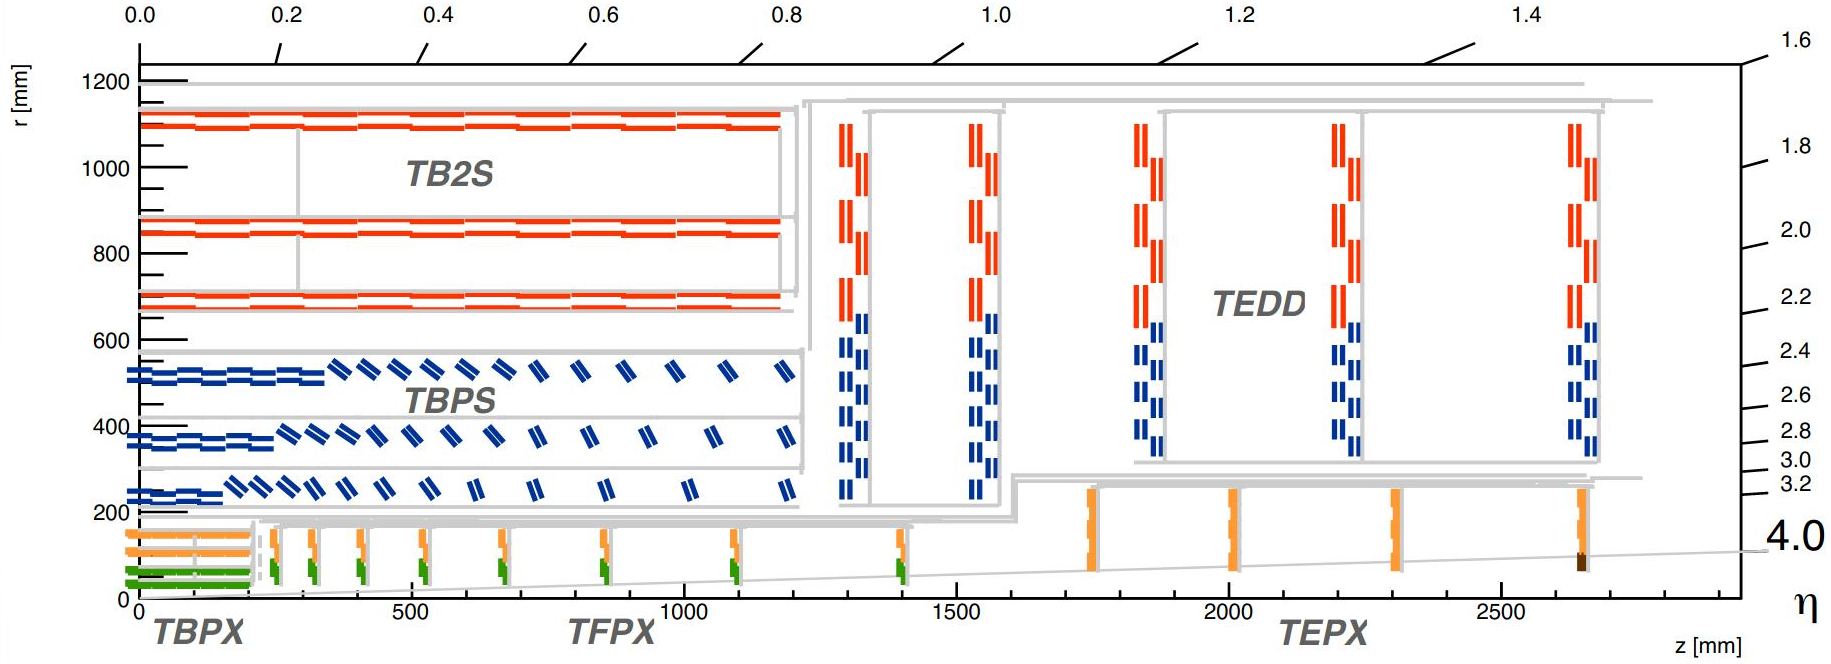
\includegraphics[width=.95\textwidth]{Cap2/imagenes/track.png}
\caption[Diagrama de una cuarta parte del diseño del detector de trazas \CMS ~ para \LHC ~ en la dirección $z$ del mismo. Los módulos de chips de lectura internos o Inner Tracker 1x2 y 2x2 se muestran en verde y amarillo respectivamente, los módulos externos o Outer Tracker PS y 2S en azul y rojo.]{Diagrama de una cuarta parte del diseño del detector de trazas \CMS ~ para HL-\LHC ~ en la dirección $z$ del detector. Los módulos de chips de lectura internos o Inner Tracker 1x2 y 2x2 se muestran en verde y amarillo respectivamente, los módulos externos o Outer Tracker PS y 2S en azul y rojo.\footnotemark.}
\label{track}
\end{figure}



El diseño esperado del detector de trazas se muestra en la Fig. \ref{track}, la región interna o \textbf{I}nner \textbf{T}racker (\textbf{IT}), donde $r < 20 ~ cm$($r < 30 ~ cm$ para $|z|> 120 ~ cm$), se espera una instrumentaria con alta granularidad detectores de píxeles que garantizan un reconocimiento de patrones eficiente en el entorno de alta densidad de pistas para la de \textbf{HL}. %La región del Rastreador externo o \textbf{OT}(\textbf{O}uter \textbf{T}racker) se instrumentará con módulos pt que proporcionan una reducción de datos en el detector aO (10) para que las mediciones precisas de las trayectorias de partículas cargadas del Rastreador se puedan usar en el disparador de Nivel 1 (L1) del Experimento CMS. 
Específicamente, las características principales del detector actualizado serán:
\footnotetext{Basada en la Fig. 1 del artículo \cite{HL_LHC_1}}
\begin{itemize}
\item Contribuir a que el disparador $L1$ mida a 40 MHz el momento de partículas cargadas y rechace aquellas con $p_T < 2 ~ GeV$.
\item Aumentar la eficiencia de detección para valores de $|\eta| < 4$ que previamente era de $|\eta| < 2.4$. 
\item Garantizar una medición precisa del momento y mantener un bajo nivel de rastreos falsos mediante una óptimización de diseño y una reducción del ``\textit{material budget}''.
\end{itemize}



\subsection{Identificación y Reconstrucción de Muones}

La identificación de partículas es parte del proceso de análisis y estudio en el \LHC, para hacer eficiente el proceso de detección, algoritmos y nuevos conceptos tuvieron que definidos e implementados para un aprovechamiento del equipamiento, con la intención de maximizar las observaciones válidas de las partículas que se estudian, en especial la identificación de procesos en los que intervienen los muones sigue siendo uno de los objetivos del proyecto por lo que se hace necesario analizar parte del proceso de identificación y reconstrucción de muones.

\subsubsection{Reconstrucción de muones.}
La reconstrucción de muones es un algoritmo sistémico que se ejecuta en un software de reconstrucción que utiliza información de impacto para rechazar objetos físicos, muones. La reconstrucción de muones se realiza en el detector de trazas y el sistema de muones, y se compone de tres pasos secuenciales: reconstrucción local, reconstrucción independiente y reconstrucción global. 

\begin{figure}[!t]
\centering
\includegraphics[width=.90\textwidth]{Cap2/imagenes/Tracking_of_Muon.png}
\caption{Probabilidad de localización de los muones en condiciones de Run-2 (izquierda) y HL (derecha).}
\label{Compara_track_muon}
\includegraphics[width=.90\textwidth]{Cap2/imagenes/Momentum_resolution_of_Muon.png}
\caption{Resolución del momento de los muones en condiciones de Run-2 (izquierda) y HL (derecha).}
\label{Compara_sol_muon}
\end{figure}
En la Fig. \ref{Compara_track_muon} se puede observar como aumenta la capacidad del experimento \CMS ~ para diferentes condiciones del experimento, en esta se evidencia el aumento de la detección de los muones con valores de $\eta > 2.4$, esto es parte del proceso de actualización a Alta Luminosidad. Además la resolución de los valores de momento reconstruidos de los muones en las condiciones actuales del experimento y en las previstas de alta luminosidad se puede ver en la Fig. \ref{Compara_sol_muon}, es clara la disminución del error para la región común ($0<\eta < 2.4$).

La reconstrucción local utiliza la información del golpe recopilada por el sistema muon para construir pistas; entonces, la información de la pista, como entrada, se alimenta al algoritmo de reconstrucción independiente. La reconstrucción global utiliza no solo información de reconstrucción independiente, sino también golpes de seguimiento de silicio. La reconstrucción del muón coincide con el camino del muón desde el sistema de muones al detector de trazas de silicio. La reconstrucción independiente se llama reconstrucción de Level-2 y la reconstrucción global se llama reconstrucción de Level-3. Los muones reconstruidos por reconstrucción independiente y global se denominan, respectivamente, muones independientes y muones globales.



\subsubsection{Identificación de muones.}

La ``D0 muon ID'' es un algoritmo utilizado para seleccionar candidatos a muones y es un algoritmo complementario para la reconstrucción estándar. A diferencia de la reconstrucción estándar, utiliza información de energía adicional de \textbf{ECAL} y \textbf{HCAL}, y está al revés en términos de información del detector. Muon Identificación primero reconstruye las pistas de los detectores de trazas de silicio y luego utiliza la información de la \textbf{ECAL} y la \textbf{HCAL}.

También se consideran los detectores que no están asociados con ningún rastro de muones independiente, lo que le permite reconstruir algunos muones de $p_\mathbf{T}$ bajos sin suficiente energía para alcanzar el sistema muónico. Estos bajos $p_\mathbf{T}$ muones pueden no ser reconstruidos como muones globales, pero son identificados por el algoritmo de identificación de muones. Los muones reconstruidos por el algoritmo de identificación se denominan muones rastreados (``tracker muons'').

\subsubsection{Aislamiento de muones}


Ya que se espera que los muones provenientes de la señal estén aislados sin depósitos sustanciales en el detector de trazas y en los calorímetros, entonces definiéndose un cono alrededor del muón como se muestra en la Fig. \ref{torre}a y considerando las posiciones del detector de trazas y calorímetro dentro de él, se calcula la energía transversal total $E_\mathbf{T}$

El muón se considera aislado si estas deposiciones no exceden algunos umbrales. La aplicación del aislamiento en la selección de muones ayuda a reducir el fondo proveniente de muchas fuentes, especialmente \textbf{QCD}, pero también de objetos pesados como $Z$ y $W+$jets 
\begin{figure}[!t]
\centering
(a)
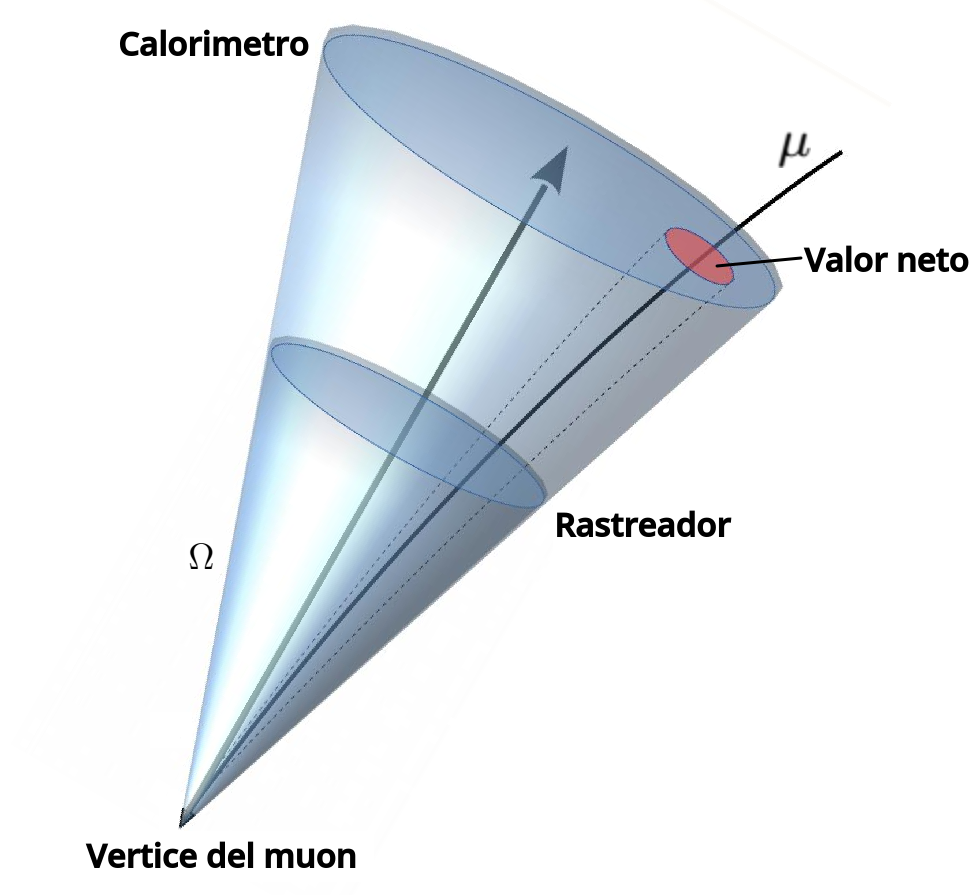
\includegraphics[width=.45\textwidth]{Cap2/imagenes/cono_mu.png}
(b)
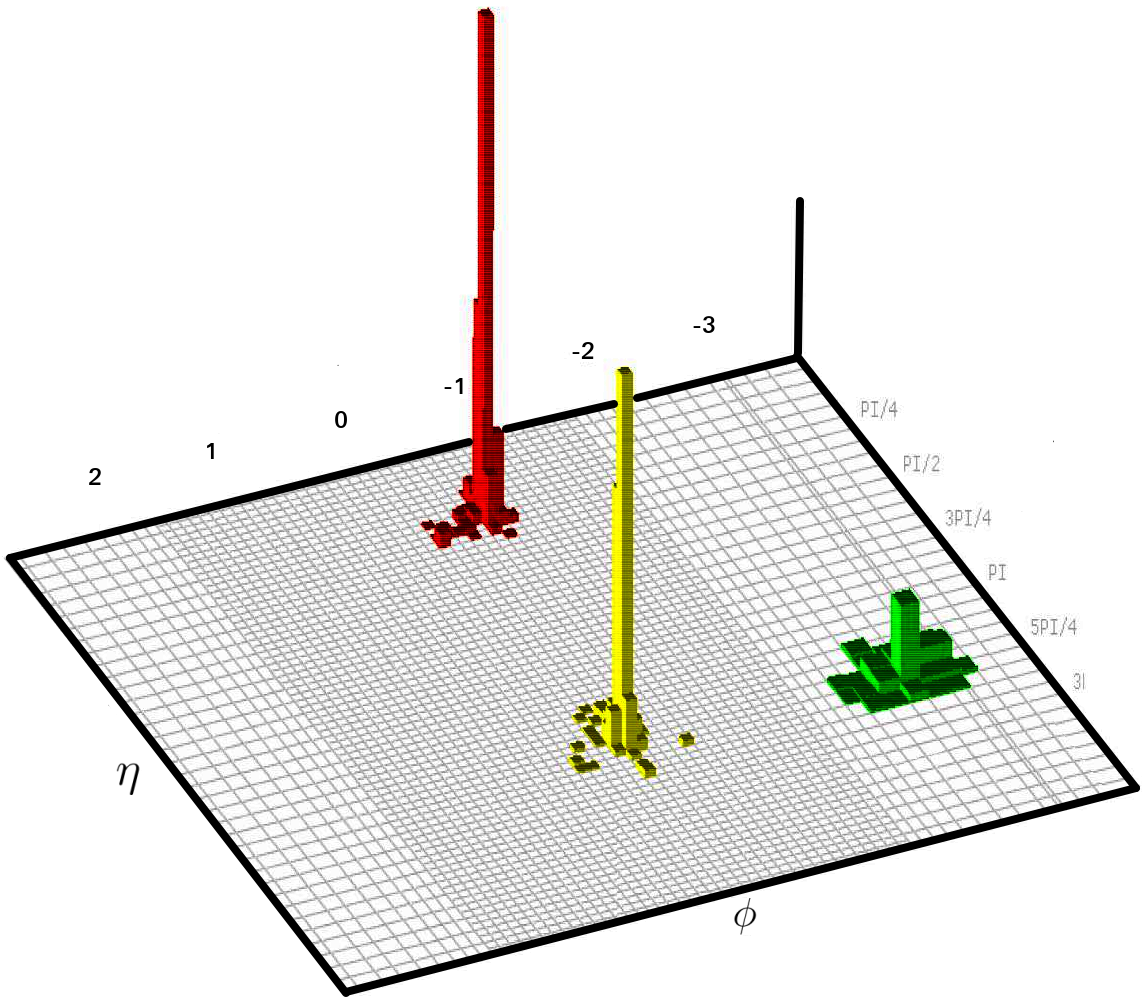
\includegraphics[width=.45\textwidth]{Cap2/imagenes/plano.png}
\caption{(a) Ilustración esquemática del cono de aislamiento. La dirección del muón en el vértice define el eje del cono; (b) Segmentación en el plano $\eta \times\phi$ en CMS sobre el que se muestran torres de energía definidas para coincidir con la segmentación o resolución del calorímetro, basada en la Fig. 1 de la referencia \cite{tower_1}.}
\label{torre}
\end{figure}
En muchas investigaciones, se han estudiado y aplicado muchos criterios de aislamiento, utilizando información de los detectores. La elección más robusta y típica realizada es aquella que contemple a todos los detectores, para tener un análisis con un criterio de aislamiento híbrido, dependiente de $p_T$, basado en una combinación de información en el detector de trazas, \textbf{HCAL} y \textbf{ECAL}. Específicamente, la variable de aislamiento basada en el detector de trazas $SumP_T$ se define como la suma escalar del $p_T$ en el plano $\eta \times \phi$ del detector de trazas dentro del cono correspondiente a $\Delta R<0.3$ donde:
\begin{equation}\label{deltaR}
\Delta R = \sqrt{\Delta \phi^2 + \Delta\eta^2}
\end{equation}
donde $\eta$ es la pseudorapidez y $\phi$ el ángulo azimutal. Entonces, alrededor del muón ($0.01 < \Delta R < 0.3$ en el plano del detector) se define como:
\begin{equation}\label{sumPT}
SumP_T =\sum_{0.01<\Delta R <0.03}^\mathbf{tracking} p_T^\mathbf{tracking}
\end{equation}
En los calorímetros, las variables $hadE_T$ y $emE_T$, correspondientes a la \textbf{HCAL} y \textbf{ECAL} respectivamente, se calculan como la suma escalar de la energía transversal depositada sobre las torres de los calorímetros (ver Fig. \ref{torre}b) en un cono de $\Delta R < 0.3$ alrededor del muón:
\begin{eqnarray}
hadE_T =\sum_{0.01<\Delta R <0.03}^\mathbf{HCAL} E_T^\mathbf{torres}  ~~~~~ y ~~~~~ emE_T =\sum_{0.01<\Delta R <0.03}^\mathbf{ECAL} E_T^\mathbf{torres} 
\end{eqnarray}
El aislamiento del detector de trazas es más importante que el de los calorimétricos, pero una combinación de los posibles aislamiento unidos a \textbf{ECAL} y \textbf{HCAL} funciona mejor. Esta combinación se construye como:
\begin{equation}\label{iso}
Iso_\mu = hadE_T + emE_T  +Sump_T
\end{equation}





\subsubsection{Eficiencia Muon}

Las secciones anteriores describen brevemente cada parte del experimento \CMS ~ desde la vía interna, más cercana a la línea del haz, hasta el sistema de muones más externo. Muchos análisis físicos requieren la probabilidad de que un muón se reconstruya como un objeto muón, dado que el muón se produce en un evento. En general, esa probabilidad se llama eficiencia, siendo la relación entre el número de muones que pasan los criterios deseados y el número total de muones producidos, se puede definir como:
\begin{equation}
\epsilon_\mu = \epsilon_\mathbf{track} \cdot \epsilon_\mathbf{id} \cdot 
\epsilon_\mathbf{iso} \cdot  \epsilon_\mathbf{trig}
\end{equation}
donde $\epsilon_\mathbf{track}$ es la eficiencia del detector de trazas de muones, es decir, la probabilidad de que un muón producido en un evento también se reconstruya%como un rastreador de silicio para detección de muones
; $\epsilon_\mathbf{id}$ es la eficiencia de identificación del muón, o sea, la probabilidad de que un muón pase por un grupo de criterios de selección, dado que es un muón reconstruido; $\epsilon_\mathbf{iso}$ es la eficiencia de aislamiento del muón, la probabilidad de que un muón reconstruido esté aislado. $\epsilon_\mathbf{trig}$ es la eficiencia del disparador, la probabilidad de que un muón reconstruido y aislado se dispare en términos de un umbral de $p_{T}$ dado.

La eficiencia de la reconstrucción muónica depende de dos factores principales: la configuración de los detectores \CMS ~ y el valor del  momento transversal $p_\mathbf{T}$ de los muones. Esta eficiencia está influenciada por la ruta a través de la cual pasa un detector, porque el detector no es homogéneo, por lo tanto, la pseudoapidez $|\eta|$ y el ángulo azimutal $\phi$ desempeñan un papel en la decisión de la eficiencia del muón. Como el detector es muy simétrico con respecto a $\phi$ no influye significativamente en la eficiencia del muón. La $p_T$ de los muones decide si tienen suficiente energía para llegar al sistema muónico, debido a que los muones independientes necesitan más de una estación para ser alcanzados en el sistema muónico, los muones con bajo $p_T$ no pueden reconstruirse como muones independientes. Toda esta información es resumida en archivos $\mathbf{*.tcl}$ característicos para uso del programa \textbf{Delphes}, aunque solo de forma básica ya que este describe de forma simplista y general el sistema.

\begin{figure}[!t]
\centering
\includegraphics[width=1\textwidth]{Cap2/imagenes/Eficiencia_of_Muon.png}
\caption{Eficiencia de reconstrucción de los muones en condiciones de Run-2 (izquierda) y HL (derecha).}
\label{Compara_eficiencia_muon}
\end{figure}


%Como se puede observar en la Fig. \ref{Compara_eficiencia_muon} se extiende como es esperado la eficiencia para valores de $\eta > 2.4$ en la configuración de Alta Luminosidad, esto como resultado de la actualización pĺanificada por el proyecto.









